\input{preamble}
\input{format}
\input{commands}

\begin{document}

\begin{Large}
    \textsf{\textbf{Homework 5}}
    
    \textbf{HDR to LDR Conversion}
\end{Large}

\vspace{1ex}

\textsf{\textbf{Student:}} \text{Yuanyuan Zhao, 2300013077, School of EECS}, \href{mailto:your.email@hotmail.com}{\texttt{zhaoyuanyuan@stu.pku.edu.cn}}\\
\textsf{\textbf{Lecturer:}} \text{Yisong Chen}
% \href{mailto:your.email@hotmail.com}
% {\texttt{chenyisong@pku.edu.cn}}\\


\vspace{2ex}


\begin{problem}{My \texttt{tonemap()}}{tonemap}
    We designed a custom \texttt{tonemap()} function that converts HDR images to LDR with reference to Matlab \texttt{tonemap()}. It processes the images by i) Luminance Extraction, ii) Log Compression, iii) Bilateral Filter Decomposition, iv) Base Layer Compression, and v) Linear Luminance Restoration. The specific implementation can be found in the file: myTonemap.mlx.

\begin{enumerate}[(a)]
    \item \textbf{Luminance Extraction}
    
        Based on CIE 1931 XYZ color space, we can calculate the luminance with the equation below which reflects human eyes' sensitivity to different colors:
        \begin{verbatim}
        L = 0.2126 * R + 0.7152 * G + 0.0722 * B;
        \end{verbatim}
   
    \item \textbf{Log Compression}
    
        Before further processing, we first compress the pixel values to log field for following reasons:
        \begin{enumerate}[label = (\roman*)]
            \item Normalize luminous variations: The variation scales of pixel values in the dark and bright regions are quite different, for instance, 0.01 vs. 100. Conversion to the log field will amplify the variations in the dark region and compress the bright one, making it easy for the subsequent filter parameter setting.
            \item Weber-Fechner law: The human eye's perception of luminance is approximately logarithmic sensitive, which corresponds to our log compression. 
        \end{enumerate}
        \begin{verbatim}
        L_log = log10(L + 1e-6);  % add 1e-6 to avoid log(0)
        \end{verbatim}

    \item \textbf{Bilateral Filter Decomposition}

        We implemented a \texttt{bilateralFilterDecomposition(I, sigma\_s, sigma\_r)} function to decompose image into base layer and detail layer (\texttt{L = baseLayer + detailLayer}) for subsequent base layer compression. Specific implementation can be found in the file: bilateralFilterDecomposition.mlx.
        \begin{enumerate}[label = (\roman*)]
            \item Generate spacial Gaussian kernel with $3 \times sigma\_s$: 
            \begin{verbatim}
            kernel_radius = ceil(3*sigma_s);
            [X, Y] = meshgrid(-kernel_radius:kernel_radius, 
                    -kernel_radius:kernel_radius);
            spatial_kernel = exp(-(X.^2 + Y.^2)/(2*sigma_s^2));
            \end{verbatim}
            \item Calculate window and luminous kernel for each pixel:
            \begin{verbatim}
            window = I(i_min:i_max, j_min:j_max);
            intensity_diff = window - I(i,j);
            intensity_kernel = exp(-(intensity_diff.^2)/(2*sigma_r^2));
            \end{verbatim}
            \item  Combine weights and normalize:
            \begin{verbatim}
            total_weight = spatial_kernel(
                                (i_min:i_max)-i+kernel_radius+1, 
                                (j_min:j_max)-j+kernel_radius+1) 
                            .* intensity_kernel;
            sum_weight = sum(total_weight(:));
            baseLayer(i,j) = sum(window(:) .* total_weight(:)) 
                            / sum_weight;
            \end{verbatim}
        \end{enumerate}
        
    \item \textbf{Base Layer Compression}

    It's the key procedure in the \texttt{tonemap()}, whose main purpose is to map the wide luminous range in the HDR image to a small one, i.e., [0, 255], to correctly display the image on common devices. We employ the compression method below:
    $$L_{compressed} = \log_{10}{\frac{10^{baseLayer} \cdot {whitePoint}}{10^{baseLayer} + {whitePoint}}}$$
    so that the $whitePoint$ can be interpreted as if the luminance is not compressed, that is, the original linear version of base layer compression:
    $$L = \frac{baseLayer \cdot whitePoint}{baseLayer + whitePoint}$$

    \item \textbf{Linear Luminance Restoration}

    The last step, combining the compressed \texttt{baseLayer} and the \texttt{detailLayer} and mapping the log field luminance to the original linear filed:
    \begin{verbatim}
    L_out = L_compressed + detailLayer;
    L_out = 10.^L_out;
    \end{verbatim}
    
    
\end{enumerate}
\end{problem}

\begin{figure}[htbp]
    \centering 
    \begin{minipage}{0.8\textwidth} 
        \centering 
        
        \begin{subfigure}[b]{0.45\linewidth} 
            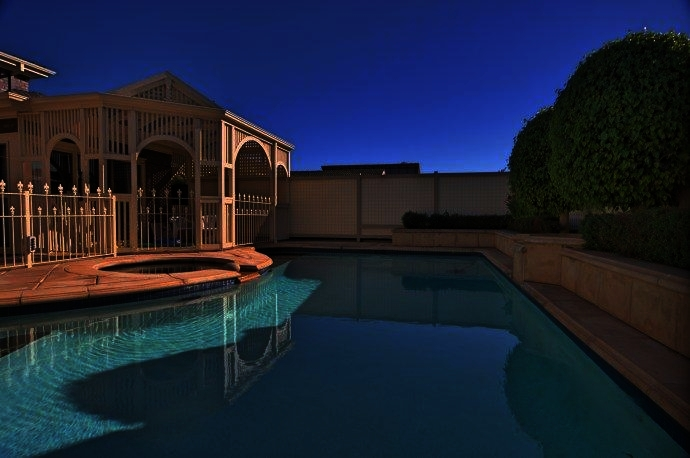
\includegraphics[width=\linewidth]{images/house_hdr.jpg}
            \caption{HDR Image}
        \end{subfigure}
        \hfill
        \begin{subfigure}[b]{0.45\linewidth}
            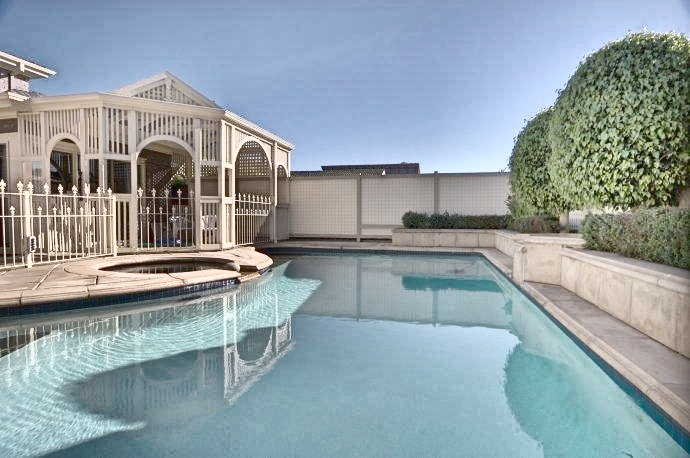
\includegraphics[width=\linewidth]{images/house_tm.jpg}
            \caption{Matlab \texttt{tonemap()}}
        \end{subfigure}

        \vspace{0.5cm}
        \begin{subfigure}[b]{0.45\linewidth}
            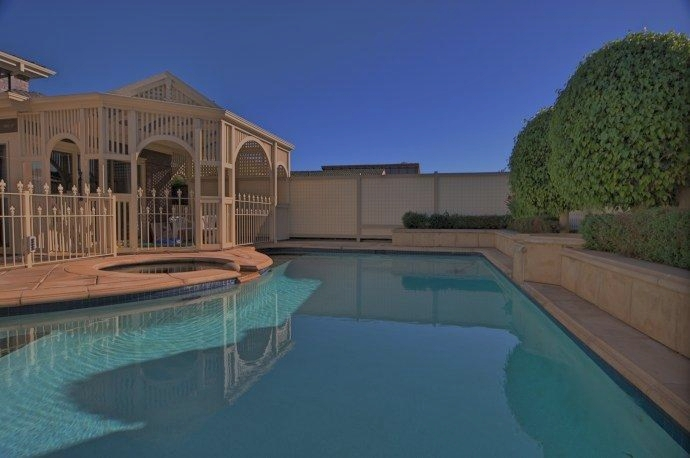
\includegraphics[width=\linewidth]{images/house_ldr.jpg}
            \caption{Custom \texttt{tonemap()} whitePoint=0.5}
        \end{subfigure}
        \hfill
        \begin{subfigure}[b]{0.45\linewidth}
            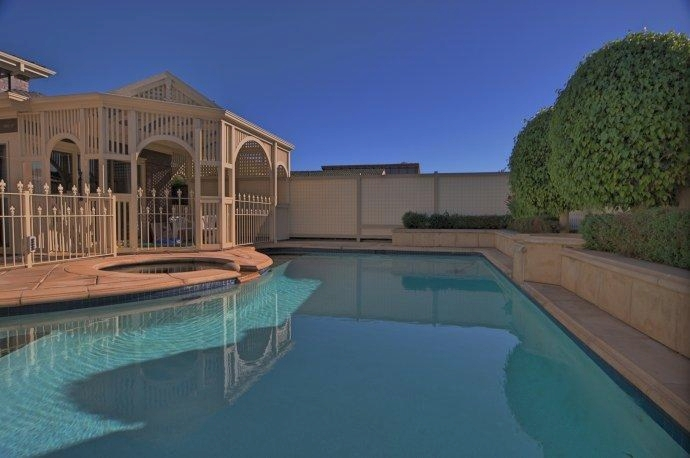
\includegraphics[width=\linewidth]{images/house_ldr_1.jpg}
            \caption{Custom \texttt{tonemap()} whitePoint=1}
        \end{subfigure}

        \caption{before and after \texttt{tonemap()}, $\gamma=2.2, \sigma_{Space}=10, \sigma_{Intensity}=0.1$}
        \label{fig:house}
    \end{minipage}
\end{figure}

\begin{figure}[htbp]
    \centering 
    \begin{minipage}{0.8\textwidth} 
        \centering 
        
        \begin{subfigure}[b]{0.45\linewidth} 
            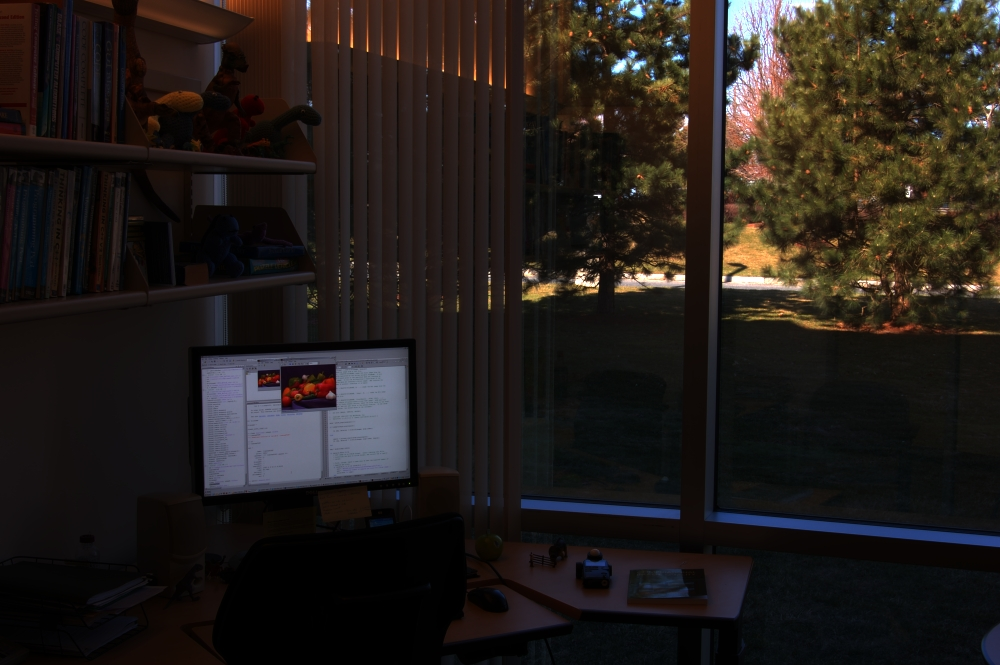
\includegraphics[width=\linewidth]{images/office_hdr.jpg}
            \caption{HDR Image}
        \end{subfigure}
        \hfill
        \begin{subfigure}[b]{0.45\linewidth}
            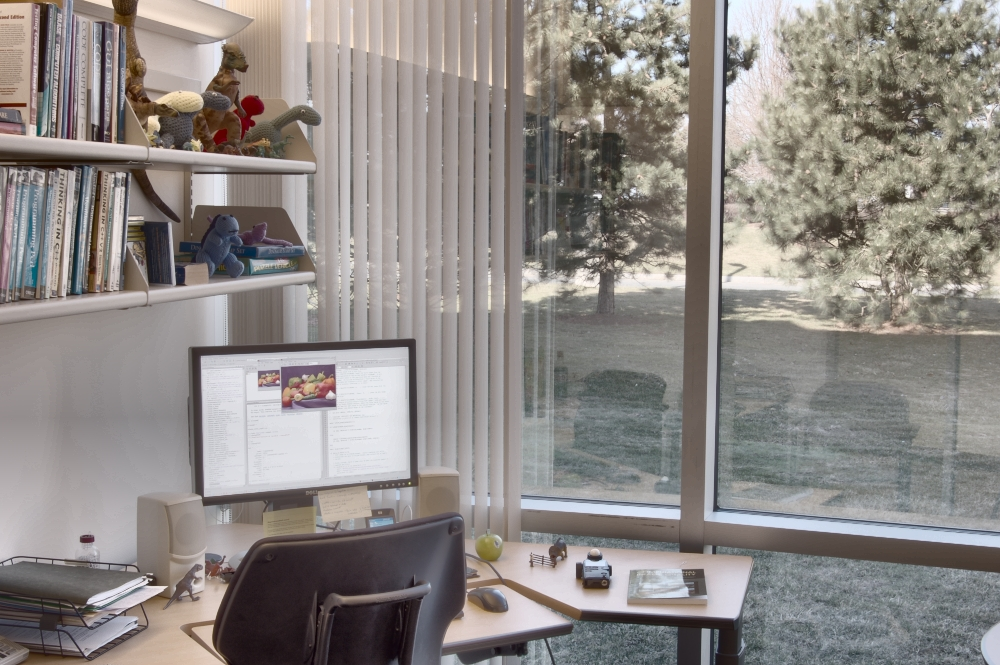
\includegraphics[width=\linewidth]{images/office_tm.jpg}
            \caption{Matlab \texttt{tonemap()}}
        \end{subfigure}

        \vspace{0.5cm}
        \begin{subfigure}[b]{0.45\linewidth}
            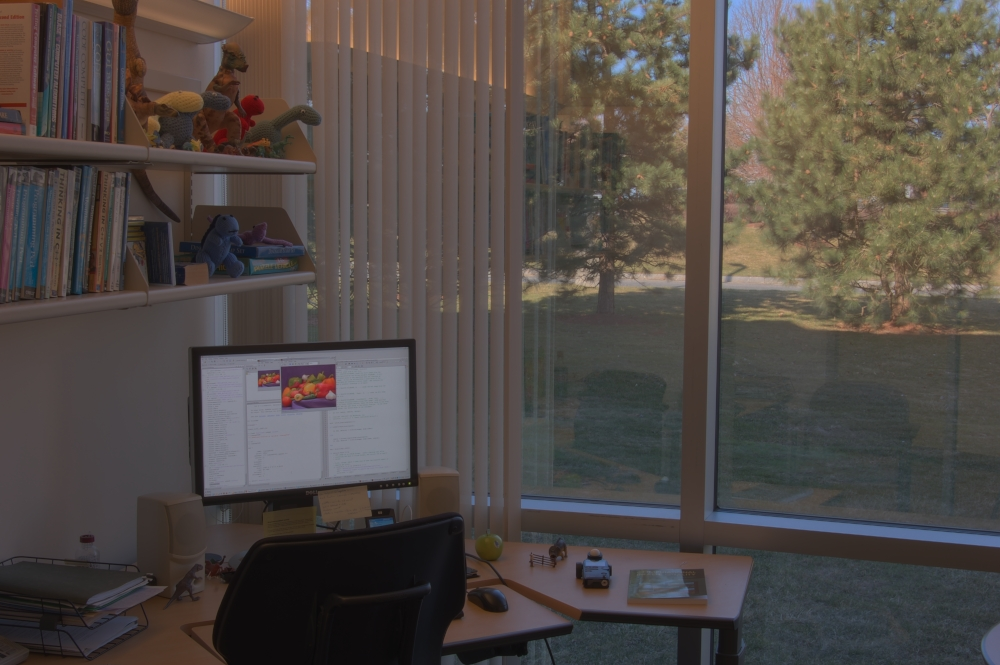
\includegraphics[width=\linewidth]{images/office_ldr.jpg}
            \caption{Custom \texttt{tonemap()} whitePoint=0.5}
        \end{subfigure}
        \hfill
        \begin{subfigure}[b]{0.45\linewidth}
            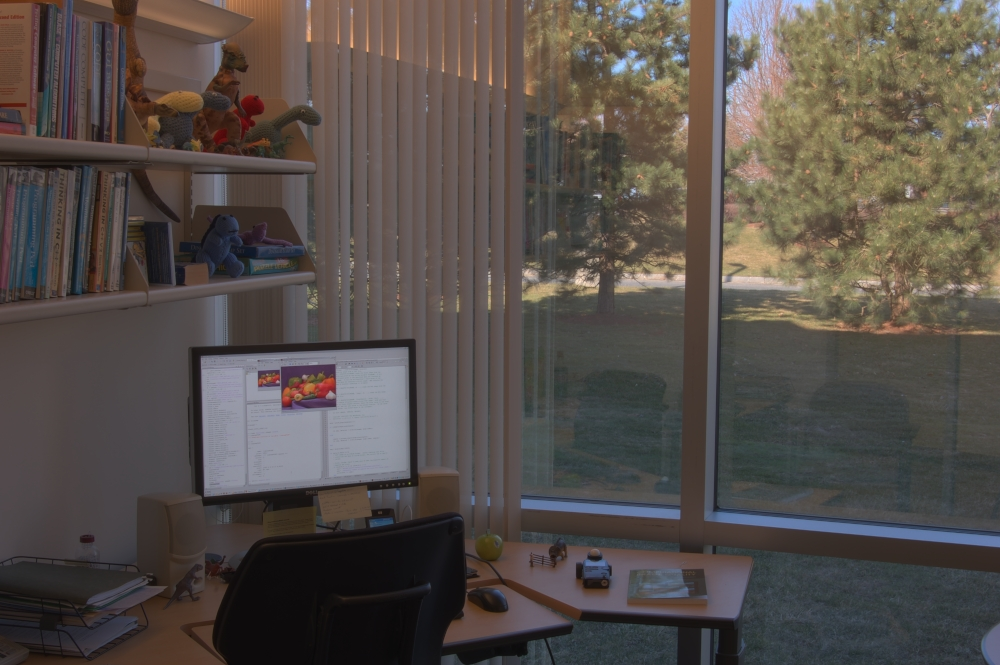
\includegraphics[width=\linewidth]{images/office_ldr_1.jpg}
            \caption{Custom \texttt{tonemap()} whitePoint=1}
        \end{subfigure}

        \caption{before and after \texttt{tonemap()}, $\gamma=2.2, \sigma_{Space}=10, \sigma_{Intensity}=0.1$}
        \label{fig:office}
    \end{minipage}
\end{figure}

\begin{figure}[htbp]
    \centering 
    \begin{minipage}{0.8\textwidth} 
        \centering 
        
        \begin{subfigure}[b]{0.45\linewidth} 
            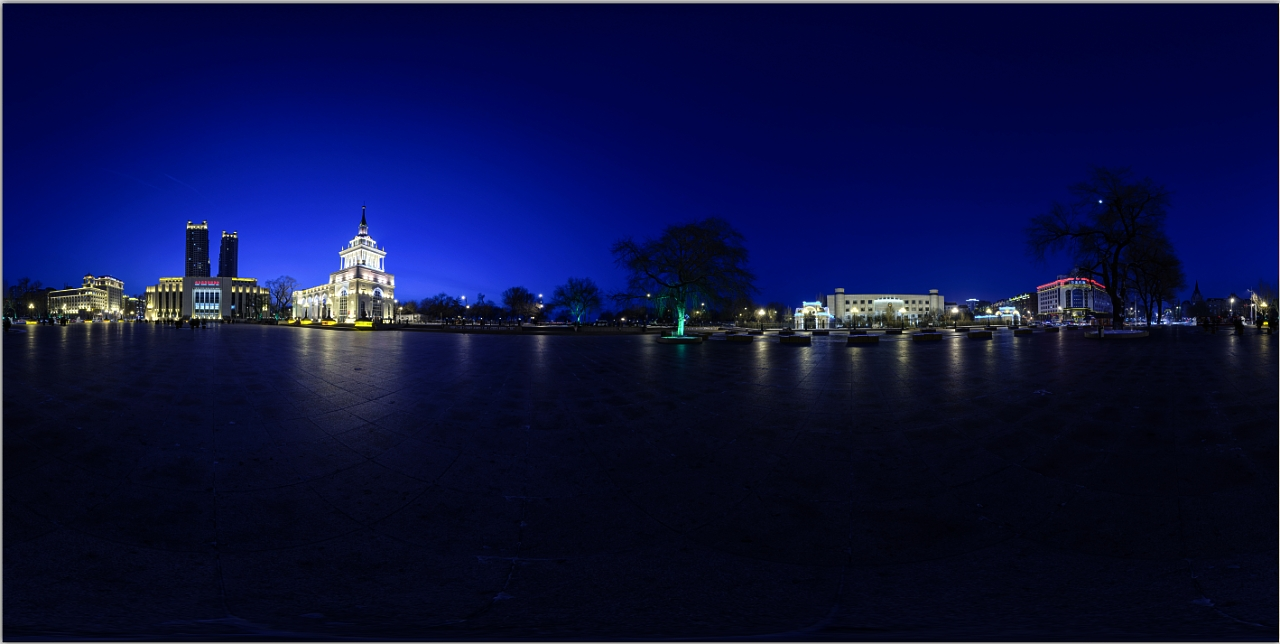
\includegraphics[width=\linewidth]{images/square_hdr.jpg}
            \caption{HDR Image}
        \end{subfigure}
        \hfill
        \begin{subfigure}[b]{0.45\linewidth}
            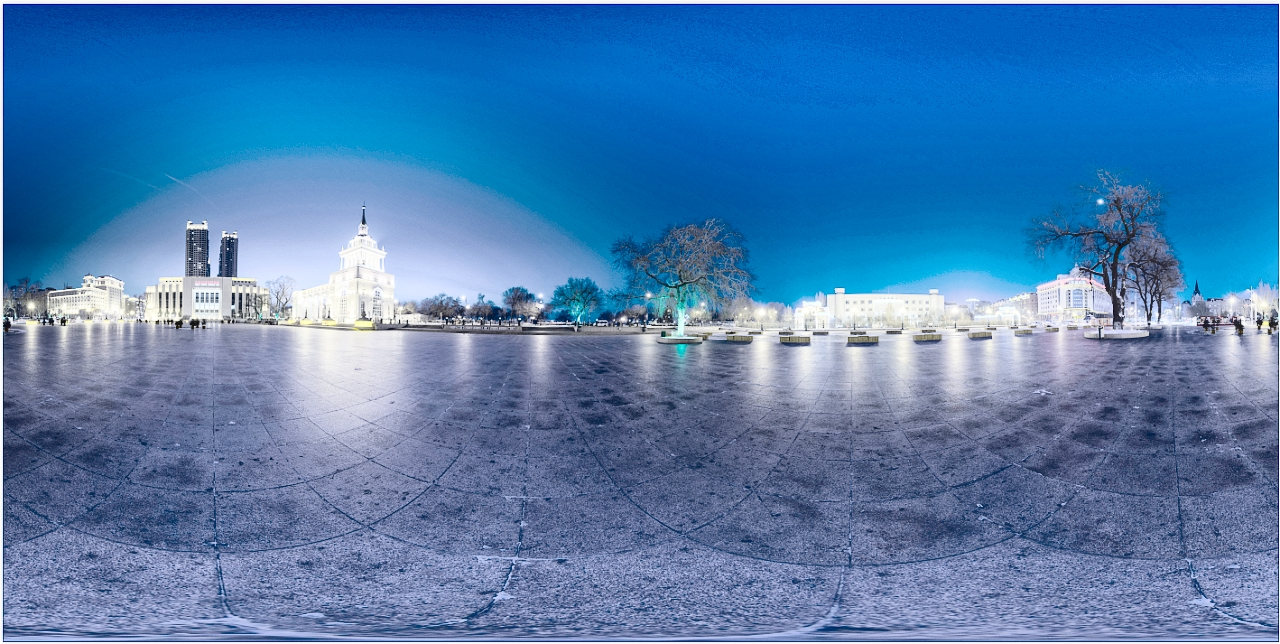
\includegraphics[width=\linewidth]{images/square_tm.jpg}
            \caption{Matlab \texttt{tonemap()}}
        \end{subfigure}

        \vspace{0.5cm}
        \begin{subfigure}[b]{0.45\linewidth}
            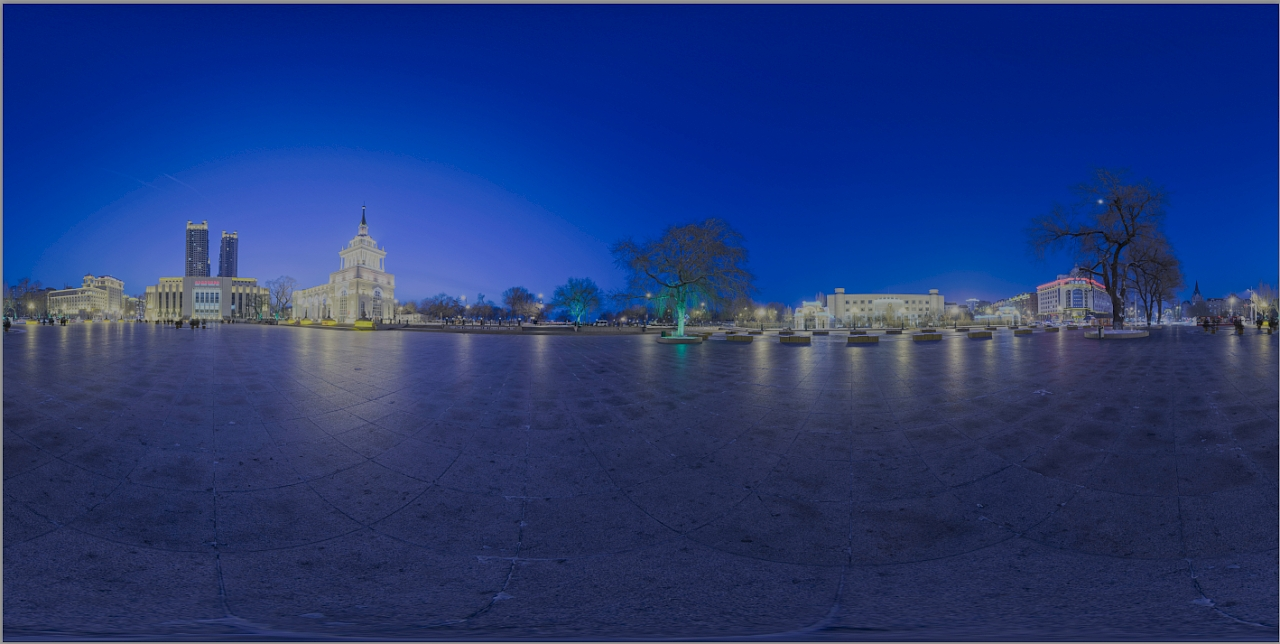
\includegraphics[width=\linewidth]{images/square_ldr.jpg}
            \caption{Custom \texttt{tonemap()} whitePoint=0.5}
        \end{subfigure}
        \hfill
        \begin{subfigure}[b]{0.45\linewidth}
            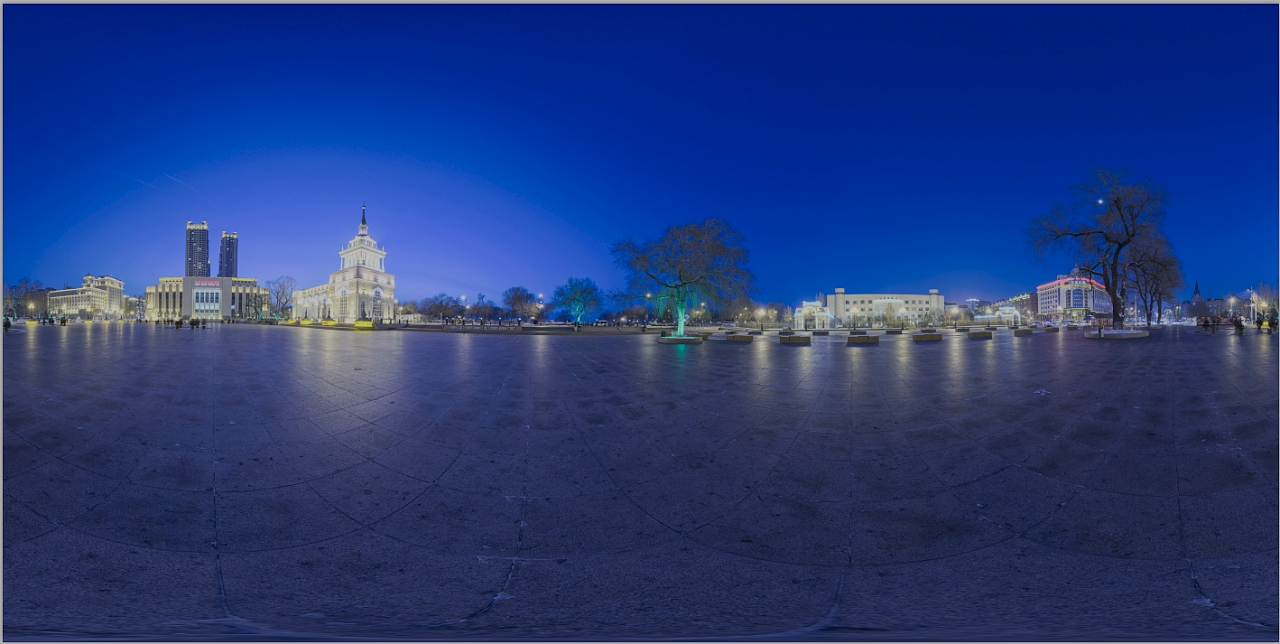
\includegraphics[width=\linewidth]{images/square_ldr_1.jpg}
            \caption{Custom \texttt{tonemap()} whitePoint=1}
        \end{subfigure}

        \caption{before and after \texttt{tonemap()}, $\gamma=2.2, \sigma_{Space}=10, \sigma_{Intensity}=0.1$}
        \label{fig:square}
    \end{minipage}
\end{figure}



\begin{problem}{Result Analysis}{result}

\begin{enumerate}[(a)]
    \item \textbf{Tone-mapped Images}\\ As shown in Figure \ref{fig:house}, \ref{fig:office}, \ref{fig:square}, the tone-mapped images are much clearer than HDR images. Thus, our custom \texttt{tonemap()} is satisfactory to a large extent.  

    \item \textbf{Matlab \texttt{tonemap()}}\\But when it comes to the differences between Matlab \texttt{tonemap()} and our custom one, it seems that the former makes the images 'whiter'. As to the reason behind this, I suppose it is because of the default parameter settings and varying compression methods.
\end{enumerate}
\end{problem}

\begin{problem}{Thoughts}{thoughts}
    The key insight of tone-map HDR conversion is to decompose basis and details and apply the compression to the former. Essentially, designing such a function is to find out a mapping from a wide luminance range to a small one. The idea of decomposition and compression is worth learning from.
\end{problem}


% =================================================

% \newpage

% \vfill

% \bibliographystyle{ieeetr}
% \bibliography{references}

\end{document}